% Options for packages loaded elsewhere
\PassOptionsToPackage{unicode}{hyperref}
\PassOptionsToPackage{hyphens}{url}
%
\documentclass[
  11pt,
  letterpaper,
]{scrbook}

\usepackage{amsmath,amssymb}
\usepackage{iftex}
\ifPDFTeX
  \usepackage[T1]{fontenc}
  \usepackage[utf8]{inputenc}
  \usepackage{textcomp} % provide euro and other symbols
\else % if luatex or xetex
  \usepackage{unicode-math}
  \defaultfontfeatures{Scale=MatchLowercase}
  \defaultfontfeatures[\rmfamily]{Ligatures=TeX,Scale=1}
\fi
\usepackage{lmodern}
\ifPDFTeX\else  
    % xetex/luatex font selection
\fi
% Use upquote if available, for straight quotes in verbatim environments
\IfFileExists{upquote.sty}{\usepackage{upquote}}{}
\IfFileExists{microtype.sty}{% use microtype if available
  \usepackage[]{microtype}
  \UseMicrotypeSet[protrusion]{basicmath} % disable protrusion for tt fonts
}{}
\makeatletter
\@ifundefined{KOMAClassName}{% if non-KOMA class
  \IfFileExists{parskip.sty}{%
    \usepackage{parskip}
  }{% else
    \setlength{\parindent}{0pt}
    \setlength{\parskip}{6pt plus 2pt minus 1pt}}
}{% if KOMA class
  \KOMAoptions{parskip=half}}
\makeatother
\usepackage{xcolor}
\setlength{\emergencystretch}{3em} % prevent overfull lines
\setcounter{secnumdepth}{5}
% Make \paragraph and \subparagraph free-standing
\ifx\paragraph\undefined\else
  \let\oldparagraph\paragraph
  \renewcommand{\paragraph}[1]{\oldparagraph{#1}\mbox{}}
\fi
\ifx\subparagraph\undefined\else
  \let\oldsubparagraph\subparagraph
  \renewcommand{\subparagraph}[1]{\oldsubparagraph{#1}\mbox{}}
\fi

\usepackage{color}
\usepackage{fancyvrb}
\newcommand{\VerbBar}{|}
\newcommand{\VERB}{\Verb[commandchars=\\\{\}]}
\DefineVerbatimEnvironment{Highlighting}{Verbatim}{commandchars=\\\{\}}
% Add ',fontsize=\small' for more characters per line
\usepackage{framed}
\definecolor{shadecolor}{RGB}{241,243,245}
\newenvironment{Shaded}{\begin{snugshade}}{\end{snugshade}}
\newcommand{\AlertTok}[1]{\textcolor[rgb]{0.68,0.00,0.00}{#1}}
\newcommand{\AnnotationTok}[1]{\textcolor[rgb]{0.37,0.37,0.37}{#1}}
\newcommand{\AttributeTok}[1]{\textcolor[rgb]{0.40,0.45,0.13}{#1}}
\newcommand{\BaseNTok}[1]{\textcolor[rgb]{0.68,0.00,0.00}{#1}}
\newcommand{\BuiltInTok}[1]{\textcolor[rgb]{0.00,0.23,0.31}{#1}}
\newcommand{\CharTok}[1]{\textcolor[rgb]{0.13,0.47,0.30}{#1}}
\newcommand{\CommentTok}[1]{\textcolor[rgb]{0.37,0.37,0.37}{#1}}
\newcommand{\CommentVarTok}[1]{\textcolor[rgb]{0.37,0.37,0.37}{\textit{#1}}}
\newcommand{\ConstantTok}[1]{\textcolor[rgb]{0.56,0.35,0.01}{#1}}
\newcommand{\ControlFlowTok}[1]{\textcolor[rgb]{0.00,0.23,0.31}{#1}}
\newcommand{\DataTypeTok}[1]{\textcolor[rgb]{0.68,0.00,0.00}{#1}}
\newcommand{\DecValTok}[1]{\textcolor[rgb]{0.68,0.00,0.00}{#1}}
\newcommand{\DocumentationTok}[1]{\textcolor[rgb]{0.37,0.37,0.37}{\textit{#1}}}
\newcommand{\ErrorTok}[1]{\textcolor[rgb]{0.68,0.00,0.00}{#1}}
\newcommand{\ExtensionTok}[1]{\textcolor[rgb]{0.00,0.23,0.31}{#1}}
\newcommand{\FloatTok}[1]{\textcolor[rgb]{0.68,0.00,0.00}{#1}}
\newcommand{\FunctionTok}[1]{\textcolor[rgb]{0.28,0.35,0.67}{#1}}
\newcommand{\ImportTok}[1]{\textcolor[rgb]{0.00,0.46,0.62}{#1}}
\newcommand{\InformationTok}[1]{\textcolor[rgb]{0.37,0.37,0.37}{#1}}
\newcommand{\KeywordTok}[1]{\textcolor[rgb]{0.00,0.23,0.31}{#1}}
\newcommand{\NormalTok}[1]{\textcolor[rgb]{0.00,0.23,0.31}{#1}}
\newcommand{\OperatorTok}[1]{\textcolor[rgb]{0.37,0.37,0.37}{#1}}
\newcommand{\OtherTok}[1]{\textcolor[rgb]{0.00,0.23,0.31}{#1}}
\newcommand{\PreprocessorTok}[1]{\textcolor[rgb]{0.68,0.00,0.00}{#1}}
\newcommand{\RegionMarkerTok}[1]{\textcolor[rgb]{0.00,0.23,0.31}{#1}}
\newcommand{\SpecialCharTok}[1]{\textcolor[rgb]{0.37,0.37,0.37}{#1}}
\newcommand{\SpecialStringTok}[1]{\textcolor[rgb]{0.13,0.47,0.30}{#1}}
\newcommand{\StringTok}[1]{\textcolor[rgb]{0.13,0.47,0.30}{#1}}
\newcommand{\VariableTok}[1]{\textcolor[rgb]{0.07,0.07,0.07}{#1}}
\newcommand{\VerbatimStringTok}[1]{\textcolor[rgb]{0.13,0.47,0.30}{#1}}
\newcommand{\WarningTok}[1]{\textcolor[rgb]{0.37,0.37,0.37}{\textit{#1}}}

\providecommand{\tightlist}{%
  \setlength{\itemsep}{0pt}\setlength{\parskip}{0pt}}\usepackage{longtable,booktabs,array}
\usepackage{calc} % for calculating minipage widths
% Correct order of tables after \paragraph or \subparagraph
\usepackage{etoolbox}
\makeatletter
\patchcmd\longtable{\par}{\if@noskipsec\mbox{}\fi\par}{}{}
\makeatother
% Allow footnotes in longtable head/foot
\IfFileExists{footnotehyper.sty}{\usepackage{footnotehyper}}{\usepackage{footnote}}
\makesavenoteenv{longtable}
\usepackage{graphicx}
\makeatletter
\def\maxwidth{\ifdim\Gin@nat@width>\linewidth\linewidth\else\Gin@nat@width\fi}
\def\maxheight{\ifdim\Gin@nat@height>\textheight\textheight\else\Gin@nat@height\fi}
\makeatother
% Scale images if necessary, so that they will not overflow the page
% margins by default, and it is still possible to overwrite the defaults
% using explicit options in \includegraphics[width, height, ...]{}
\setkeys{Gin}{width=\maxwidth,height=\maxheight,keepaspectratio}
% Set default figure placement to htbp
\makeatletter
\def\fps@figure{htbp}
\makeatother
\newlength{\cslhangindent}
\setlength{\cslhangindent}{1.5em}
\newlength{\csllabelwidth}
\setlength{\csllabelwidth}{3em}
\newlength{\cslentryspacingunit} % times entry-spacing
\setlength{\cslentryspacingunit}{\parskip}
\newenvironment{CSLReferences}[2] % #1 hanging-ident, #2 entry spacing
 {% don't indent paragraphs
  \setlength{\parindent}{0pt}
  % turn on hanging indent if param 1 is 1
  \ifodd #1
  \let\oldpar\par
  \def\par{\hangindent=\cslhangindent\oldpar}
  \fi
  % set entry spacing
  \setlength{\parskip}{#2\cslentryspacingunit}
 }%
 {}
\usepackage{calc}
\newcommand{\CSLBlock}[1]{#1\hfill\break}
\newcommand{\CSLLeftMargin}[1]{\parbox[t]{\csllabelwidth}{#1}}
\newcommand{\CSLRightInline}[1]{\parbox[t]{\linewidth - \csllabelwidth}{#1}\break}
\newcommand{\CSLIndent}[1]{\hspace{\cslhangindent}#1}

% \usepackage{amsmath,amssymb,mathtools}
\usepackage{enumerate}
\usepackage{geometry}
\geometry{hmargin=1.2in}

\usepackage{booktabs}
\usepackage{amssymb}
\makeatletter
\def\thm@space@setup{%
  \thm@preskip=8pt plus 2pt minus 4pt
  \thm@postskip=\thm@preskip
}
\makeatother

\usepackage{framed,color}
\definecolor{shadecolor}{RGB}{248,248,248}

\renewcommand{\textfraction}{0.05}
\renewcommand{\topfraction}{0.8}
\renewcommand{\bottomfraction}{0.8}
\renewcommand{\floatpagefraction}{0.75}

%\let\oldhref\href
%\renewcommand{\href}[2]{#2\footnote{\url{#1}}}

\ifxetex
  \usepackage{letltxmacro}
  \setlength{\XeTeXLinkMargin}{1pt}
  \LetLtxMacro\SavedIncludeGraphics\includegraphics
  \def\includegraphics#1#{% #1 catches optional stuff (star/opt. arg.)
    \IncludeGraphicsAux{#1}%
  }%
  \newcommand*{\IncludeGraphicsAux}[2]{%
    \XeTeXLinkBox{%
      \SavedIncludeGraphics#1{#2}%
    }%
  }%
\fi

\makeatletter
\newenvironment{kframe}{%
\medskip{}
\setlength{\fboxsep}{.8em}
 \def\at@end@of@kframe{}%
 \ifinner\ifhmode%
  \def\at@end@of@kframe{\end{minipage}}%
  \begin{minipage}{\columnwidth}%
 \fi\fi%
 \def\FrameCommand##1{\hskip\@totalleftmargin \hskip-\fboxsep
 \colorbox{shadecolor}{##1}\hskip-\fboxsep
     % There is no \\@totalrightmargin, so:
     \hskip-\linewidth \hskip-\@totalleftmargin \hskip\columnwidth}%
 \MakeFramed {\advance\hsize-\width
   \@totalleftmargin\z@ \linewidth\hsize
   \@setminipage}}%
 {\par\unskip\endMakeFramed%
 \at@end@of@kframe}
\makeatother

\makeatletter
\@ifundefined{Shaded}{
}{\renewenvironment{Shaded}{\begin{kframe}}{\end{kframe}}}
\makeatother

\newenvironment{rmdblock}[1]
  {
  \begin{itemize}
  \renewcommand{\labelitemi}{
    \raisebox{-.7\height}[0pt][0pt]{
      {\setkeys{Gin}{width=3em,keepaspectratio}\includegraphics{images/#1}}
    }
  }
  \setlength{\fboxsep}{1em}
  \begin{kframe}
  \item
  }
  {
  \end{kframe}
  \end{itemize}
  }
\newenvironment{rmdnote}
  {\begin{rmdblock}{note}}
  {\end{rmdblock}}
\newenvironment{rmdcaution}
  {\begin{rmdblock}{caution}}
  {\end{rmdblock}}
\newenvironment{rmdimportant}
  {\begin{rmdblock}{important}}
  {\end{rmdblock}}
\newenvironment{rmdtip}
  {\begin{rmdblock}{tip}}
  {\end{rmdblock}}
\newenvironment{rmdwarning}
  {\begin{rmdblock}{warning}}
  {\end{rmdblock}}
\usepackage{mathrsfs}
\DeclareMathAlphabet{\mathcrl}{U}{rsfs}{m}{n}
\usepackage{utopia}
\DeclareMathAlphabet{\mathcal}{OMS}{cmsy}{m}{n}
\makeatletter
\makeatother
\makeatletter
\@ifpackageloaded{bookmark}{}{\usepackage{bookmark}}
\makeatother
\makeatletter
\@ifpackageloaded{caption}{}{\usepackage{caption}}
\AtBeginDocument{%
\ifdefined\contentsname
  \renewcommand*\contentsname{Table of contents}
\else
  \newcommand\contentsname{Table of contents}
\fi
\ifdefined\listfigurename
  \renewcommand*\listfigurename{List of Figures}
\else
  \newcommand\listfigurename{List of Figures}
\fi
\ifdefined\listtablename
  \renewcommand*\listtablename{List of Tables}
\else
  \newcommand\listtablename{List of Tables}
\fi
\ifdefined\figurename
  \renewcommand*\figurename{Figure}
\else
  \newcommand\figurename{Figure}
\fi
\ifdefined\tablename
  \renewcommand*\tablename{Table}
\else
  \newcommand\tablename{Table}
\fi
}
\@ifpackageloaded{float}{}{\usepackage{float}}
\floatstyle{ruled}
\@ifundefined{c@chapter}{\newfloat{codelisting}{h}{lop}}{\newfloat{codelisting}{h}{lop}[chapter]}
\floatname{codelisting}{Listing}
\newcommand*\listoflistings{\listof{codelisting}{List of Listings}}
\usepackage{amsthm}
\theoremstyle{definition}
\newtheorem{definition}{Definition}[chapter]
\theoremstyle{definition}
\newtheorem{example}{Example}[chapter]
\theoremstyle{remark}
\AtBeginDocument{\renewcommand*{\proofname}{Proof}}
\newtheorem*{remark}{Remark}
\newtheorem*{solution}{Solution}
\makeatother
\makeatletter
\@ifpackageloaded{caption}{}{\usepackage{caption}}
\@ifpackageloaded{subcaption}{}{\usepackage{subcaption}}
\makeatother
\makeatletter
\@ifpackageloaded{tcolorbox}{}{\usepackage[skins,breakable]{tcolorbox}}
\makeatother
\makeatletter
\@ifundefined{shadecolor}{\definecolor{shadecolor}{rgb}{.97, .97, .97}}
\makeatother
\makeatletter
\makeatother
\makeatletter
\makeatother
\ifLuaTeX
  \usepackage{selnolig}  % disable illegal ligatures
\fi
\IfFileExists{bookmark.sty}{\usepackage{bookmark}}{\usepackage{hyperref}}
\IfFileExists{xurl.sty}{\usepackage{xurl}}{} % add URL line breaks if available
\urlstyle{same} % disable monospaced font for URLs
\hypersetup{
  pdftitle={Bayesian modelling},
  pdfauthor={Léo Belzile},
  hidelinks,
  pdfcreator={LaTeX via pandoc}}

\title{Bayesian modelling}
\author{Léo Belzile}
\date{}

\begin{document}
\frontmatter
\maketitle
\ifdefined\Shaded\renewenvironment{Shaded}{\begin{tcolorbox}[borderline west={3pt}{0pt}{shadecolor}, frame hidden, interior hidden, sharp corners, boxrule=0pt, enhanced, breakable]}{\end{tcolorbox}}\fi

\renewcommand*\contentsname{Table of contents}
{
\setcounter{tocdepth}{2}
\tableofcontents
}
\mainmatter
\bookmarksetup{startatroot}

\hypertarget{welcome}{%
\chapter*{Welcome}\label{welcome}}
\addcontentsline{toc}{chapter}{Welcome}

\markboth{Welcome}{Welcome}

This book is a web complement to MATH 80601A \emph{Bayesian modelling},
a graduate course offered at HEC Montréal.

These notes are licensed under a
\href{http://creativecommons.org/licenses/by-nc-sa/4.0/}{Creative
Commons Attribution-NonCommercial-ShareAlike 4.0 International License}
and were last compiled on Thursday, August 24 2023.

The objective of the course is to provide a hands on introduction to
Bayesian data analysis. The course will cover the formulation,
evaluation and comparison of Bayesian models through examples and
real-data applications.

\bookmarksetup{startatroot}

\hypertarget{introduction}{%
\chapter{Introduction}\label{introduction}}

\hypertarget{bayes-theorem}{%
\section{Bayes theorem}\label{bayes-theorem}}

Denote by \(p(X) \equiv\Pr(X)\) denotes the marginal density of \(X\),
\(p(X \mid Y)\) the conditional of \(X\) given \(Y\) and \(p(X, Y)\) the
joint density. Bayes' theorem states that \begin{align*}
p(X = x \mid Y=y) = \frac{p(Y = y \mid X = x)p(X=x)}{p(Y=y)}
\end{align*}

In the case of discrete random variable \(X\) with support
\(\mathcal{X},\) the denominator can be evaluated using the law of total
probability as
\[\Pr(Y=y) = \sum_{x \in \mathcal{X}}\Pr(Y =y \mid X=x)\Pr(X=x).\]

\begin{example}[]\protect\hypertarget{exm-covidrapidtest}{}\label{exm-covidrapidtest}

Back in January 2021, the Quebec government was debating whether or not
to distribute antigen rapid test, with
\href{https://www.cbc.ca/news/canada/montreal/quebec-avoids-relying-on-rapid-covid-19-tests-as-pressure-mounts-to-follow-ontario-s-lead-1.5896738}{strong
reluctance} from authorities given the paucity of available resources
and the poor sensitivity.

A Swiss study analyse the efficiency of rapid antigen tests, comparing
them to repeated polymerase chain reaction (PCR) test output, taken as
benchmark (\protect\hyperlink{ref-Jegerlehner:2021}{Jegerlehner et al.
2021}). The results are presented in Table~\ref{tbl-covid19}

\hypertarget{tbl-covid19}{}
\begin{longtable}[]{@{}lrr@{}}
\caption{\label{tbl-covid19}Confusion matrix of Covid test results for
PCR tests versus rapid antigen tests, from Jegerlehner et al.
(\protect\hyperlink{ref-Jegerlehner:2021}{2021}).}\tabularnewline
\toprule\noalign{}
& PCR \(+\) & PCR \(-\) \\
\midrule\noalign{}
\endfirsthead
\toprule\noalign{}
& PCR \(+\) & PCR \(-\) \\
\midrule\noalign{}
\endhead
\bottomrule\noalign{}
\endlastfoot
rapid \(+\) & 92 & 2 \\
rapid \(-\) & 49 & 1319 \\
total & 141 & 1321 \\
\end{longtable}

Estimated seropositivity at the end of January 2021 according to
projections of the Institute for Health Metrics and Evaluation (IHME) of
8.18M out of 38M inhabitants
(\protect\hyperlink{ref-owidcoronavirus}{Mathieu et al. 2020}), a
prevalence of 21.4\%. Assuming the latter holds uniformly over the
country, what is the probability of having Covid if I get a negative
result to a rapid test?

Let \(R^{-}\) (\(R^{+}\)) denote a negative (positive) rapid test result
and \(C^{+}\) (\(C^{-}\)) Covid positivity (negativity). Bayes' formula
gives \begin{align*}
\Pr(C^{+} \mid R^{-}) & = \frac{\Pr(R^{-} \mid C^{+})\Pr(C^{+})}{\Pr(R^{-} \mid C^{+})\Pr(C^{+}) + \Pr(R^{-} \mid C^{-})\Pr(C^{-})} \\&=
\frac{49/141 \cdot 0.214}{49/141 \cdot 0.214 + 1319/1321 \cdot 0.786}
\end{align*} so there is a small, but non-negligible probability of
8.66\% that the rapid test result is misleading. Jegerlehner et al.
(\protect\hyperlink{ref-Jegerlehner:2021}{2021}) indeed found that the
sensitivity was 65.3\% among symptomatic individuals, but dropped down
to 44\% for asymptomatic cases. This may have fueled government experts
skepticism.

\end{example}

\hypertarget{probability-and-frequency}{%
\section{Probability and frequency}\label{probability-and-frequency}}

In classical (frequentist) parametric statistic, we treat observations
\(\boldsymbol{Y}\) as realizations of a distribution whose parameters
\(\boldsymbol{\theta}\) are unknown. All of the information about
parameters is encoded by the likelihood function, which is optimized
numerically or analytically to find the maximum likelihood estimator.
Large-sample theory shows that the resulting estimator is asymptotically
normal under regularity conditions.

The interpretation of probability in the classical statistic is
understood in terms of long run frequency, which is why we call this
approach frequentist statistic. Think of a fair die: when we state that
values \(\{1, \ldots, 6\}\) are equiprobable, we mean that repeatedly
tossing the die should result, in large sample, in each outcome being
realized roughly \(1/6\) of the time (the symmetry of the object also
implies that each facet should be equally likely to lie face up). This
interpretation also carries over to confidence intervals: a
\((1-\alpha)\) confidence interval either contains the true parameter
value or it doesn't, so the probability level \((1-\alpha)\) is only the
long-run proportion of intervals created by the procedure that should
contain the true fixed value, not the probability that a single interval
contains the true value. This is counter-intuitive to most.

In practice, the true value of the parameter \(\boldsymbol{\theta}\)
vector is unknown to the practitioner, thus uncertain: Bayesians would
argue that we should treat the latter as a random quantity rather than a
fixed constant. Since different people may have different knowledge
about these potential values, the prior knowledge is a form of
\textbf{subjective probability}. For example, if you play cards, one
person may have recorded the previous cards that were played, whereas
other may not. They thus assign different probability of certain cards
being played. In Bayesian inference, we consider \(\boldsymbol{\theta}\)
as random variables to reflect our lack of knowledge about potential
values taken. Italian scientist Bruno de Finetti, who is famous for the
claim ``Probability does not exist'\,', stated in the preface of Finetti
(\protect\hyperlink{ref-deFinetti:1974}{1974}):

\begin{quote}
Probabilistic reasoning --- always to be understood as subjective ---
merely stems from our being uncertain about something. It makes no
difference whether the uncertainty relates to an unforseeable future, or
to an unnoticed past, or to a past doubtfully reported or forgotten: it
may even relate to something more or less knowable (by means of a
computation, a logical deduction, etc.) but for which we are not willing
or able tho make the effort; and so on {[}\ldots{]} The only relevant
thing is uncertainty --- the extent of our knowledge and ignorance. The
actual fact of whether or not the events considered are in some sense
\emph{determined}, or known by other people, and so on, is of no
consequence.
\end{quote}

On page 3, de Finetti continues
(\protect\hyperlink{ref-deFinetti:1974}{Finetti 1974})

\begin{quote}
only subjective probabilities exist --- i.e., the degree of belief in
the occurrence of an event attributed by a given person at a given
instant and with a given set of information.
\end{quote}

The likelihood
\(\mathcal{L}(\boldsymbol{\theta}; \boldsymbol{y}) \equiv p(\boldsymbol{y} \mid \boldsymbol{\theta})\)
is the starting point for Bayesian inference. However, we adjoin to it a
\textbf{prior} distribution \(p(\boldsymbol{\theta})\) that reflects the
prior knowledge about potential values taken by the \(p\)-dimensional
parameter vector, before observing the data \(\boldsymbol{y}\). We thus
seek \(p(\boldsymbol{\theta} \mid \boldsymbol{y})\): the observations
are random variables but inference is performed conditional on the
observed sample. By Bayes' theorem, the posterior distribution
\(p(\boldsymbol{\Theta} \mid \boldsymbol{Y})\) is

\begin{equation}\protect\hypertarget{eq-posterior}{}{
p(\boldsymbol{\Theta} \mid \boldsymbol{Y}) = \frac{p(\boldsymbol{Y} \mid \boldsymbol{\Theta}) p(\boldsymbol{\Theta})}{\int p(\boldsymbol{Y} \mid \boldsymbol{\theta}) p(\boldsymbol{\theta}) \mathrm{d} \boldsymbol{\theta}},
}\label{eq-posterior}\end{equation}

so the posterior \(p(\boldsymbol{\theta} \mid \boldsymbol{y})\) is
proportional, as a function of \(\theta,\) to the product of the
likelihood and the prior function. The integral in the denominator,
termed marginal likelihood and denoted
\(p(\boldsymbol{Y}) = \mathsf{E}_{\boldsymbol{\theta}}\{p(\boldsymbol{Y} \mid \boldsymbol{\theta})\}\),
is a normalizing constant that makes the right hand side integrate to
unity.

For the posterior to be \textbf{proper}, we need the product on the
right hand side to be integrable. The denominator of
Equation~\ref{eq-posterior} is a normalizing constant so that the
posterior is a distribution. If \(\boldsymbol{\theta}\) is low
dimensional, numerical integration such as quadrature methods can be
used to compute the latter. To obtain the marginal posterior,
\[p(\theta_j \mid \boldsymbol{y}) = \int p(\boldsymbol{\theta} \mid \boldsymbol{y}) \mathrm{d} \boldsymbol{\theta}_{-j},\]
additional integration is needed.

Consider a binomial likelihood with probability of success \(p\) and
\(n\) trials, \(Y \sim \mathsf{Bin}(n, p)\). If we take a beta prior,
\(p \sim \mathsf{Be}(\alpha, \beta)\) and observe \(k\) successes, the
posterior is \begin{align*}
p(\theta \mid y = k) &\propto \binom{n}{k} p^k (1-p)^{n-k} \frac{\Gamma(\alpha + \beta)}{\Gamma(\alpha) \Gamma(\beta)}p^{\alpha-1} (1-p)^{\beta-1}
\\&\stackrel{p}{\propto} p^{k+\alpha-1}(1-p)^{n-k+\beta-1}
\end{align*} and is
\[\int_{0}^{1} p^{k+\alpha-1}(1-p)^{n-k+\beta-1}\mathrm{d} p = \frac{\Gamma(k+\alpha)\Gamma(n-k+\beta)}{\Gamma(n+\alpha+\beta)},\]
a Beta function. Since we need only to keep track of the terms that are
function of the parameter \(p\), we could recognize directly that the
posterior distribution is \(\mathsf{Be}(k+\alpha, n-k+\beta)\) and
deduce the normalizing constant from there.

The number of success should be roughly \(np\) and the number of
failures \(n(1-p)\) and so the likelihood contribution, relative to the
prior, will dominate as the sample size \(n\) grows.

Another way to see this is to track moments (expectation, variance,
etc.) The Beta distribution, whose density is
\(f(x; \alpha, \beta) \propto x^{\alpha-1} (1-x)^{\beta-1}\), has
expectation \(\alpha/(\alpha+\beta)\) and variance
\(\alpha\beta/\{(\alpha+\beta)^2(\alpha+\beta+1)\}\) and so as
\(n \to \infty\), the mean of the posterior will be dominated by
information from the likelihood. An alternative parametrization takes
\(\alpha=\mu \kappa\), \(\beta = (1-\mu)\kappa\) for \(\mu \in (0,1)\)
and \(\kappa>0\), so that the model is parametrized directly in terms of
mean \(\mu\).

\begin{figure}[ht!]

{\centering 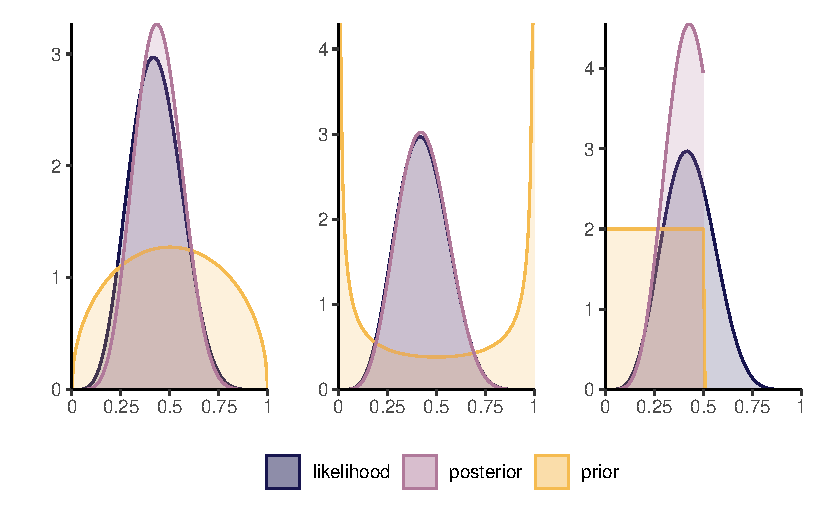
\includegraphics{introduction_files/figure-pdf/fig-betabinom-1.pdf}

}

\caption{\label{fig-betabinom}Binomial likelihood for six successes out
of 14 trials, \(\mathsf{Beta}(3/2, 3/2)\) prior and posterior
distribution from a beta-binomial model. The posterior curve is much
closer to the likelihood than it is to the prior, even with a relatively
small sample size.}

\end{figure}

While a density integrates to 1 over the range of possible outcomes, the
likelihood function does not when we integrate over the range of the
parameters.

The beta-binomial model is an example of conjugate model, meaning the
posterior distribution is from the same family as the prior.\footnote{This
  is a property of exponential families that will be revisited in the
  next chapter.} While we could calculate analytically the value of the
normalizing constant, we could also for arbitrary priors use numerical
integration in the event the parameter vector \(\boldsymbol{\theta}\) is
low-dimensional. For a single scalar \(p\) on the unit interval,
numerical integration or Monte Carlo integration yield nearly identical
results.

\begin{Shaded}
\begin{Highlighting}[]
\NormalTok{k }\OtherTok{\textless{}{-}}\NormalTok{ 6L }\CommentTok{\# number of successes }
\NormalTok{n }\OtherTok{\textless{}{-}}\NormalTok{ 14L }\CommentTok{\# number of trials}
\NormalTok{alpha }\OtherTok{\textless{}{-}}\NormalTok{ beta }\OtherTok{\textless{}{-}} \FloatTok{1.5} \CommentTok{\# prior parameters}
\NormalTok{unnormalized\_posterior }\OtherTok{\textless{}{-}} \ControlFlowTok{function}\NormalTok{(p)\{}
\NormalTok{  p}\SpecialCharTok{\^{}}\NormalTok{(k}\SpecialCharTok{+}\NormalTok{alpha}\DecValTok{{-}1}\NormalTok{) }\SpecialCharTok{*}\NormalTok{ (}\DecValTok{1}\SpecialCharTok{{-}}\NormalTok{p)}\SpecialCharTok{\^{}}\NormalTok{(n}\SpecialCharTok{{-}}\NormalTok{k }\SpecialCharTok{+}\NormalTok{ beta }\SpecialCharTok{{-}} \DecValTok{1}\NormalTok{)}
\NormalTok{\}}
\FunctionTok{integrate}\NormalTok{(}\AttributeTok{f =}\NormalTok{ unnormalized\_posterior,}
          \AttributeTok{lower =} \DecValTok{0}\NormalTok{,}
          \AttributeTok{upper =} \DecValTok{1}\NormalTok{)}
\end{Highlighting}
\end{Shaded}

\begin{verbatim}
1.066906e-05 with absolute error < 1e-12
\end{verbatim}

\begin{Shaded}
\begin{Highlighting}[]
\CommentTok{\# Compare with known constant}
\FunctionTok{beta}\NormalTok{(k }\SpecialCharTok{+}\NormalTok{ alpha, n }\SpecialCharTok{{-}}\NormalTok{ k }\SpecialCharTok{+}\NormalTok{ beta)}
\end{Highlighting}
\end{Shaded}

\begin{verbatim}
[1] 1.066906e-05
\end{verbatim}

\begin{Shaded}
\begin{Highlighting}[]
\CommentTok{\# Monte Carlo integration}
\FunctionTok{mean}\NormalTok{(}\FunctionTok{unnormalized\_posterior}\NormalTok{(}\FunctionTok{runif}\NormalTok{(}\FloatTok{1e5}\NormalTok{)))}
\end{Highlighting}
\end{Shaded}

\begin{verbatim}
[1] 1.064055e-05
\end{verbatim}

\begin{Shaded}
\begin{Highlighting}[]
\CommentTok{\# Alternative approach, sampling from the prior}
\CommentTok{\# This is less efficient}
\FunctionTok{mean}\NormalTok{(}\FunctionTok{dbinom}\NormalTok{(}\AttributeTok{x =}\NormalTok{ k, }
            \AttributeTok{size =}\NormalTok{ n, }
            \AttributeTok{prob =} \FunctionTok{rbeta}\NormalTok{(}\AttributeTok{n =} \FloatTok{1e6}\NormalTok{, alpha, beta))) }\SpecialCharTok{*}
  \FunctionTok{beta}\NormalTok{(alpha, beta) }\SpecialCharTok{/} \FunctionTok{choose}\NormalTok{(n, k)}
\end{Highlighting}
\end{Shaded}

\begin{verbatim}
[1] 1.065653e-05
\end{verbatim}

When \(\boldsymbol{\theta}\) is high-dimensional, the marginal
likelihood is untractable. This is one of the main challenges of
Bayesian statistics and the popularity and applicability has grown
drastically with the development and popularity of numerical algorithms,
following th publication of Geman and Geman
(\protect\hyperlink{ref-Geman.Geman:1984}{1984}) and Gelfand and Smith
(\protect\hyperlink{ref-Gelfand.Smith:1990}{1990}). Markov chain Monte
Carlo methods circumvent the calculation of the denominator by drawing
approximate samples from the posterior.

\hypertarget{bayesian-updating}{%
\subsection{Bayesian updating}\label{bayesian-updating}}

Subjective probabilities imply that different people with different
prior beliefs would arrive at different conclusions. However, as more
data are gathered, we can use Bayes theorem to update these prior
beliefs and update the posterior. In most instances, the relative weight
of the prior relative to the likelihood becomes negligible: if we
consider independent data \(\boldsymbol{y}_1, \boldsymbol{y}_n\)
observed sequentially, then \begin{align*}
p(\boldsymbol{\theta} \mid \boldsymbol{y}_1, \ldots, \boldsymbol{y}_k) &\stackrel{\boldsymbol{\theta}}{\propto} p(\boldsymbol{y}_k \mid \boldsymbol{\theta}) p(\boldsymbol{\theta} \mid \boldsymbol{y}_1, \ldots, \boldsymbol{y}_{k-1})
\\ & \stackrel{\boldsymbol{\theta}}{\propto} \prod_{i=1}^k p(\boldsymbol{y}_i \mid \boldsymbol{\theta}) p(\boldsymbol{\theta})
\end{align*} If data are exchangeable, the order in which observations
are collected and the order of the belief updating is irrelevant to the
full posterior
\(p(\boldsymbol{\theta} \mid \boldsymbol{y}_1, \ldots \boldsymbol{y}_n)\).

\bookmarksetup{startatroot}

\hypertarget{priors}{%
\chapter{Priors}\label{priors}}

The posterior distribution combines two ingredients: the likelihood and
the prior. If the former is a standard ingredient of any
likelihood-based inference, prior specification requires some care. The
purpose of this chapter is to consider different standard way of
constructing prior functions.

\hypertarget{conjugate-priors}{%
\section{Conjugate priors}\label{conjugate-priors}}

A distribution belongs to an exponential family with parameter vector
\(\boldsymbol{\theta} \in \mathbb{R}^D\) if it can be written as
\begin{align*}
f(y; \boldsymbol{\theta}) = \exp\left\{ \sum_{k=1}^K Q_k(\boldsymbol{\theta}) t_k(y) + D(\boldsymbol{\theta})\right\}
\end{align*} and in particular, the support does not depend on unknown
parameters. If we have an independent and identically distributed sample
of observations \(y_1, \ldots, y_n\), the log likelihood is thus of the
form \begin{align*}
\ell(\boldsymbol{\theta}) = \sum_{k=1}^K \phi_k(\boldsymbol{\theta}) \sum_{i=1}^n t_k(y_i) + n D(\boldsymbol{\theta}),
\end{align*} where the collection \(\sum_{i=1}^n t_k(y_i)\)
(\(k=1, \ldots, K\)) are sufficient statistics and
\(\phi_k(\boldsymbol{\theta})\) are the canonical parameters. The number
of sufficient statistics are the same regardless of the sample size.
Exponential families play a prominent role in generalized linear models,
in which the natural parameters are modelled as linear function of
explanatories.

A log prior density that is proportional to \begin{align*}
\log p(\boldsymbol{\theta}) \propto \eta D(\boldsymbol{\theta}) + \sum_{k=1}^K Q_k(\boldsymbol{\theta}) \nu_k
\end{align*} is conjugate.

\begin{example}[Conjugate priors for the binomial
model]\protect\hypertarget{exm-conjugatepriors-binom}{}\label{exm-conjugatepriors-binom}

The binomial log density with \(y\) successes out of \(n\) trials is
proportional to \begin{align*}
y \log(p) + (n-y) \log(1-p) = y\log\left( \frac{p}{1-p}\right) + n \log(1-p)
\end{align*} with canonical parameter \(\mathrm{logit}(p)\), which is
the natural link function for Bernoulli, giving rise to logistic
regresion model.

Since the density of the binomial is of the form \(p^y(1-p)^{n-y}\), the
beta distribution \(\mathsf{Be}(\alpha, \beta)\) with density
\(f(x) \propto x^{\alpha-1} (1-x)^{\beta-1}\) is the conjugate prior.

The posterior mean \begin{align*}
 \mathsf{E}(p \mid y) = w\frac{y}{n} + (1-w) \frac{a}{a+b}, 
 \qquad w = \frac{n}{n+a+b}
 \end{align*} is therefore a weighted average of the maximum likelihood
estimator and the prior mean. We can think of the parameter \(\alpha\)
(respectively \(\beta\)) as representing the prior number of success
(resp. failures).

\end{example}

\begin{example}[Conjugate prior for the Poisson
model]\protect\hypertarget{exm-conjugatepriors-poisson}{}\label{exm-conjugatepriors-poisson}

The Poisson distribution with mean \(\mu\) has log density proportional
to \(f(y; \mu) \propto y\log(\mu) -\mu\), so is an exponential family
with natural parameter \(\log(\mu)\). The gamma distribution,
\(p(x) \propto \beta^{\alpha}/\Gamma(\alpha)x^{\alpha-1} \exp(-\beta x)\)
with shape \(\alpha\) and rate \(\beta\) is the conjugate prior for the
Poisson. For an \(n\)-sample of independent observations
\(\mathsf{Po}(\mu)\) observations with
\(\mu \sim \mathsf{Ga}(\alpha, \beta)\), the posterior is
\(\mathsf{Ga}(\sum_{i=1}^n y_i + \alpha, \beta + n)\).

\end{example}

\begin{example}[Posterior rates for A/B tests using conjugate Poisson
model]\protect\hypertarget{exm-abtest}{}\label{exm-abtest}

Upworthy.com, a US media publisher, revolutionized headlines online
advertisement by running systematic A/B tests to compare the different
wording of headlines, placement and image and what catches attention the
most. The Upworthy Research Archive
(\protect\hyperlink{ref-Matias:2021}{Matias et al. 2021}) contains
results for 22743 experiments, with a click through rate of 1.58\% on
average and a standard deviation of 1.23\%. The
\texttt{clickability\_test\_id} gives the unique identifier of the
experiment, \texttt{clicks} the number of conversion out of
\texttt{impressions}. See
\href{https://tellingstorieswithdata.com/08-hunt.html\#ab-testing}{Section
8.5} of Alexander (\protect\hyperlink{ref-Alexander:2023}{2023}) for
more details about A/B testing and background information.

Consider an A/B test from November 23st, 2014, that compared four
different headlines for a story on Sesame Street workshop with
interviews of children whose parents were in jail and visiting them in
prisons. The headlines tested were:

\begin{quote}
\begin{enumerate}
\def\labelenumi{\arabic{enumi}.}
\tightlist
\item
  Some Don't Like It When He Sees His Mom. But To Him? Pure Joy. Why
  Keep Her From Him?
\item
  They're Not In Danger. They're Right. See True Compassion From The
  Children Of The Incarcerated.
\item
  Kids Have No Place In Jail \ldots{} But In This Case, They
  \emph{Totally} Deserve It.
\item
  Going To Jail \emph{Should} Be The Worst Part Of Their Life. It's So
  Not. Not At All.
\end{enumerate}
\end{quote}

At first glance, the first and third headlines seem likely to lead to a
curiosity gap. The wording of the second is more explicit (and
searchable), whereas the first is worded as a question.

We model the conversion rate \(\lambda_i\) for each headline separately
using a Poisson distribution and compare the posterior distributions for
all four choices. Using a conjugate prior and selecting the parameters
by moment matching yields approximately \(\alpha = 1.64\) and
\(\beta = 0.01\) for the hyperparameters.

\hypertarget{tbl-upworthy}{}
\begin{longtable}[]{@{}lrr@{}}
\caption{\label{tbl-upworthy}Number of views, clicks for different
headlines for the Upworthy data.}\tabularnewline
\toprule\noalign{}
headline & impressions & clicks \\
\midrule\noalign{}
\endfirsthead
\toprule\noalign{}
headline & impressions & clicks \\
\midrule\noalign{}
\endhead
\bottomrule\noalign{}
\endlastfoot
H1 & 3060 & 49 \\
H2 & 2982 & 20 \\
H3 & 3112 & 31 \\
H4 & 3083 & 9 \\
\end{longtable}

\begin{figure}[ht!]

{\centering 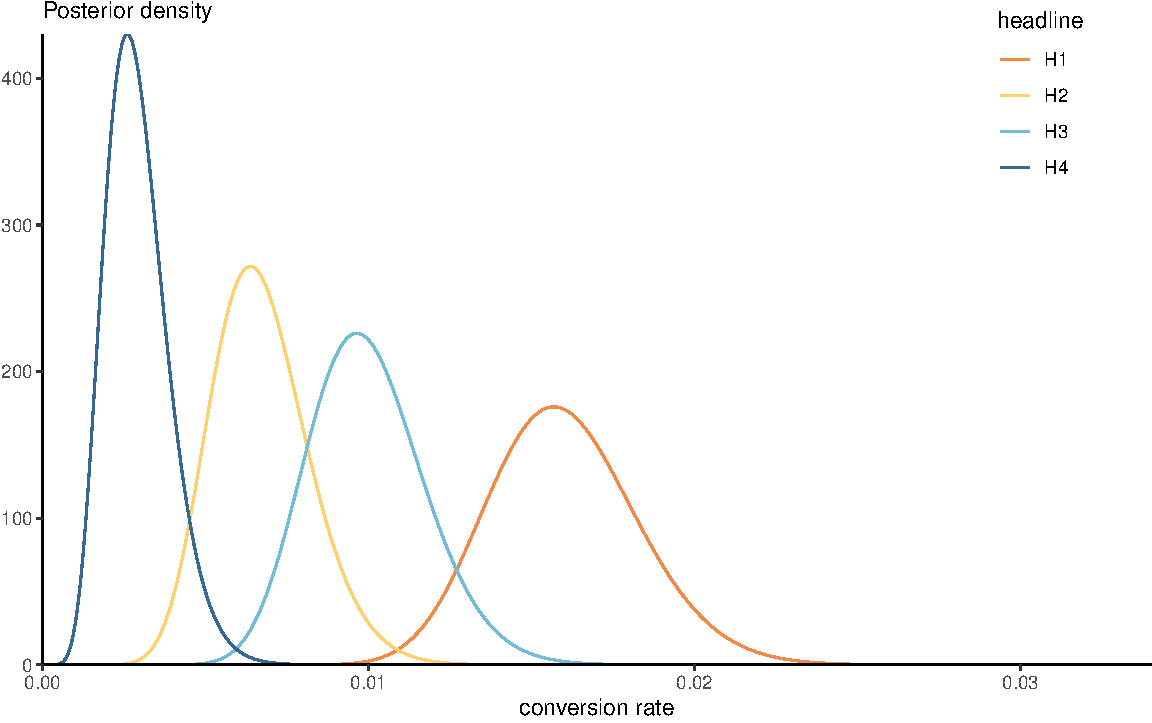
\includegraphics{priors_files/figure-pdf/fig-upworthy-1.pdf}

}

\caption{\label{fig-upworthy}Gamma posterior for the Upworthy Sesame
street headline.}

\end{figure}

We can visualize the posterior distributions. In this context, the large
sample size lead to the dominance of the likelihood contribution
\(p(Y_i \mid \lambda_i) \sim \mathsf{Po}(n_i\lambda_i)\) relative to the
prior. We can see there is virtually no overlap between different rates
for headers H1 (preferred) relative to H4 (least favorable). The
probability that Headline 3 is better than Headline 1 can be
approximated by simulating samples from both posterior and computing the
proportion of times one is larger: the probability of superiority is
1.7\%, indicating a clear preference for the first headline \texttt{H1}.

\end{example}

\begin{example}[Conjugate priors in the Bayesian linear
model]\protect\hypertarget{exm-conjugatepriors-normal}{}\label{exm-conjugatepriors-normal}

Consider a linear regression model with observation-specific mean
\(\mu_i = \mathbf{x}_i\boldsymbol{\beta}\) \((i=1,\ldots, n)\) with
\(\mathbf{x}_i\) the \(i\)th row of the \(n \times p\) design matrix
\(\mathbf{X}\).

Concatenating records,
\(\boldsymbol{Y} \sim \mathsf{No}_n(\mathbf{X}\boldsymbol{\beta}, \sigma^2 \mathbf{Q}_y^{-1})\),
for a known precision matrix \(\mathbf{Q}_y\), typically
\(\mathbf{I}_n\). To construct a conjugate joint prior for
\(p(\boldsymbol{\beta}, \sigma^2)\), we consider the sequential
formulation \begin{align*}
\boldsymbol{\beta} \mid \sigma^2 \sim \mathsf{No}_p(\boldsymbol{\nu}_\beta, \sigma^2 \mathbf{Q}^{-1}_\beta), \qquad \sigma^2 \sim \mathsf{IG}(\alpha,\beta)
\end{align*} where \(\mathsf{IG}\) denotes the inverse gamma
distribution\footnote{This simply means that the precision
  \(\sigma^{-2}\), the reciprocal of the variance, has a gamma
  distribution with shape \(\alpha\) and rate \(\beta\).}

The joint posterior is Gaussian-inverse gamma and can be factorized
\begin{align*}
p(\boldsymbol{\beta}, \sigma^2 \mid y) = p(\sigma^2 \mid y) p(\boldsymbol{\beta} \mid \sigma^2, y)
\end{align*} where
\(p(\sigma^2 \mid y) \sim \mathsf{IG}(\alpha^*, \beta^*)\) and
\(p(\boldsymbol{\beta} \mid \sigma^2, y) \sim \mathsf{No}_p(\mathbf{M}\boldsymbol{m}, \sigma^2\mathbf{M})\)
with \(\alpha^* = \alpha + n/2\),
\(\beta^*=\beta + 0.5 \boldsymbol{\nu}_\beta^\top \mathbf{Q}_\beta\boldsymbol{\nu}_\beta + \boldsymbol{y}^\top\boldsymbol{y} - \boldsymbol{m}^\top\mathbf{M}\boldsymbol{m}\),
\(\boldsymbol{m} = \mathbf{Q}_\beta \boldsymbol{\nu}_\beta + \mathbf{X}^\top \mathbf{Q}_y\boldsymbol{y}\)
and
\(\mathbf{M} = (\mathbf{Q}_\beta + \mathbf{X}^\top\mathbf{Q}_y\mathbf{X})^{-1}\);
the latter can be evaluated efficiently using
Shermann--Morrisson--Woodbury identity.

\end{example}

The exponential family is quite large;
\href{https://doi.org/10.1.1.157.5540}{Fink (1997) \emph{A Compendium of
Conjugate Priors}} gives multiple examples of conjugate priors and work
out parameter values.

One criticism of the Bayesian approach is the arbitrariness of prior
functions. However, the role of the prior is often negligible in large
samples (consider for example the posterior of exponential families with
conjugate priors). Moreover, the likelihood is also chosen for
convenience, and arguably has a bigger influence on the conclusion. Data
fitted using a linear regression model seldom follow Gaussian
distributions conditionally, in the same way that the linearity is a
convenience (and first order approximation).

In general, unless the sample size is small and we want to add expert
opinion, we may wish to pick an \emph{uninformative prior}, i.e., one
that does not impact much the outcome. For conjugate models, one can
often show that the relative weight of prior parameters (relative to the
random sample likelihood contribution) becomes negligible by
\href{https://en.wikipedia.org/wiki/Conjugate_prior}{investigating their
relative weights}.

\hypertarget{uninformative-priors}{%
\section{Uninformative priors}\label{uninformative-priors}}

\begin{definition}[Proper
prior]\protect\hypertarget{def-properprior}{}\label{def-properprior}

We call a prior \emph{proper} if it's integral is finite; such prior
function automatically leads to a valid posterior.

\end{definition}

The best example of prior priors arise from probability density
function. We can still employ this rule for improper priors: for
example, taking \(\alpha, \beta \to 0\) in the beta prior leads to a
prior proportional to \(x^{-1}(1-x)^{-1}\), the integral of which
diverges on the unit interval \([0,1]\). However, as long as the number
of success and the number of failures is larger than 1, meaning
\(k \geq 1, n-k \geq 1\), the posterior distribution would be proper,
i.e., integrable. To find the posterior, normalizing constants are also
superfluous.

Many uninformative priors are flat, or proportional to a uniform on some
subset of the real line and therefore improper. It may be superficially
tempting to set a uniform prior on a large range to ensure posterior
property, but the major problem is that a flat prior may be informative
in a different parametrization, as the following example suggests.

\begin{example}[]\protect\hypertarget{exm-scaleflatprior}{}\label{exm-scaleflatprior}

Consider the parameter \(\log(\tau) \in \mathbb{R}\) and the prior
\(p( \log \tau) \propto 1\). If we reparametrize the model in terms of
\(\tau\), the new prior (including the Jacobian of the transformation)
is \(\tau^{-1}\)

\end{example}

Some priors are standard and widely used. In location scale families
with location \(\nu\) and scale \(\tau\), the density is such that
\begin{align*}
f(x; \nu, \tau) =  \frac{1}{\tau} f\left(\frac{x - \nu}{\tau}\right), \qquad \nu \in \mathbb{R}, \tau >0.
\end{align*} We thus wish to have a prior so that
\(p(\tau) = c^{-1}p(\tau/c)\) for any scaling \(c>0\), whence it follows
that \(p(\tau) \propto \tau^{-1}\), which is uniform on the log scale.

The priors \(p(\nu) \propto 1\) and \(p(\tau) \propto \tau^{-1}\) are
both improper but lead to location and scale invariance, hence that the
result is the same regardless of the units of measurement.

\begin{definition}[Jeffrey's
prior]\protect\hypertarget{def-jeffreys}{}\label{def-jeffreys}

In single parameter models, taking a prior function for \(\theta\)
proportional to the square root of the determinant of the information
matrix \(p(\theta) \propto \imath(\theta)\) yields a prior that is
invariant to parametrization, so that inferences conducted in different
parametrizations are equivalent.

To see this, consider a bijective transformation
\(\theta \mapsto \vartheta\). Under the reparametrized model and
suitable regularity conditions\footnote{Using Bartlett's identity;
  Fisher consistency can be established using the dominated convergence
  theorem.}, the chain rule implies that \begin{align*}
i(\vartheta) &= - \mathsf{E} \left(\frac{\partial^2 \ell(\vartheta)}{\partial^2 \vartheta}\right)
\\&= - \mathsf{E}\left(\frac{\partial^2 \ell(\theta)}{\partial \theta^2}\right) \left( \frac{\mathrm{d} \theta}{\mathrm{d} \vartheta} \right)^2 + \mathsf{E}\left(\frac{\partial \ell(\theta)}{\partial \theta}\right) \frac{\mathrm{d}^2 \theta}{\mathrm{d} \vartheta^2}
\end{align*} Since the score has mean zero,
\(\mathsf{E}\left\{\partial \ell(\theta)/\partial \theta\right\}=0\),
the rightmost term vanishes. We can thus relate the Fisher information
in both parametrizations, with \begin{align*}
\imath^{1/2}(\vartheta) = \imath^{1/2}(\theta) \left| \frac{\mathrm{d} \theta}{\mathrm{d} \vartheta} \right|,
\end{align*} implying invariance.

Most of the times, Jeffrey's prior is improper. For the binomial model,
it can be viewed as a limiting conjugate beta prior with
\(\alpha, \beta\to 0\)). Unfortunately, in multiparameter models, the
system isn't invariant to reparametrization if we consider the
determinant of the Fisher information.

\end{definition}

\begin{example}[]\protect\hypertarget{exm-jeffreysbinom}{}\label{exm-jeffreysbinom}

Consider the binomial distribution
\(f(y; \theta, n) \propto \theta^y(1-\theta)^{n-y}\mathsf{I}_{\theta \in [0,1]}\).
The negative of the second derivative of the log likelihood with respect
to \(p\) is
\(\jmath(\theta) = - \partial^2 \ell(\theta; y) / \partial \theta^2 = y/\theta^2 + (1-y)/(1-\theta)^2\)
and since \(\mathsf{E}(Y)=n\theta\), thus the Fisher information is
\(\imath = \mathsf{E}\{\jmath(\theta)\}=n/\theta + n/(1-\theta) = n/\{\theta(1-\theta)\}\).\footnote{The
  Fisher information is linear in the sample size for independent and
  identically distributed data.}

Jeffrey's prior is thus
\(p(\theta) \propto \theta^{-1}(1-\theta)^{-1}\).

\end{example}

\leavevmode\vadjust pre{\hypertarget{exer-jeffreysnormal}{}}%
Check that for the Gaussian distribution \(\mathsf{No}(\mu, \sigma^2)\),
the Jeffrey's prior obtained by treating each parameter in turn, fixing
the value of the other, are \(p(\mu) \propto 1\) and
\(p(\sigma) \propto 1/\sigma\), which also correspond to the default
uninformative priors for location-scale families.

\begin{example}[]\protect\hypertarget{exm-jeffreyspoisson}{}\label{exm-jeffreyspoisson}

The Poisson distribution with
\(\ell(\lambda) \propto -\lambda + y\log \lambda\), with second
derivative
\(-\partial^2 \ell(\lambda)/\partial \lambda^2 = y/\lambda^2\). Since
the mean of the Poisson distribution is \(\lambda\), the Fisher
information is \(\imath(\lambda) = \lambda^{-1}\) and Jeffrey's prior is
\(\lambda^{-1/2}\).

\end{example}

\hypertarget{expert-knowledge}{%
\section{Expert knowledge}\label{expert-knowledge}}

Th prior distribution may have parameters themselves that need to be
specified by experts. One may also wish to add another layer and set an
hyperprior distribution on the parameters, resulting in a hierarchical
model.

Setting parameters of priors is often done by reparametrizing the latter
in terms of moments. Sometimes, it may be easier to set priors in a
different scale where subject-matter expertise is most easily elicited.

\begin{example}[]\protect\hypertarget{exm-colestawn}{}\label{exm-colestawn}

The generalized extreme value distribution arises as the limiting
distribution for the maximum of \(m\) independent observations. The
\(\mathsf{GEV}(\mu, \sigma, \xi)\) distribution is a location-scale with
distribution function \begin{align*}
F(x) = \exp\left\{ - \left(1+\xi(x-\mu)/\sigma\right)^{-1/\xi}_{+}\right\}
\end{align*} where \(x_{+} = \max\{0, x\}\).

Inverting the distribution function yields the quantile function
\begin{align*}
Q(p) \mu + \sigma \frac{(-\log p)^{-\xi}-1}{\xi}
\end{align*}

In environmental data, we often model annual maximum. Engineering
designs are often specified in terms of the \(k\)-year return levels,
defined as the quantile of the annual maximum exceeded with probability
\(1/k\) in any given year. Using a \(\mathsf{GEV}\) for annual maximum,
Coles and Tawn (\protect\hyperlink{ref-Coles.Tawn:1996}{1996}) proposed
modelling annual daily rainfall and specifying a prior on the quantile
scale \(q_1 < q_2 < q_3\) for tail probabilities \(p_1> p_2 > p_3\). To
deal with the ordering constraints, gamma priors are imposed on the
differences \(q_1 - o \sim \mathsf{Ga}(\alpha_1, \beta_1)\),
\(q_2 - q_1 \sim \mathsf{Ga}(\alpha_2, \beta_2)\) and
\(q_3-q_2 \sim \mathsf{Ga}(\alpha_3, \beta_3)\), where \(o\) is the
lower bound of the support. The prior is thus of the form

\begin{align*}
p(\boldsymbol{q}) \propto q_1^{\alpha_1-1}\exp(-\beta_1 q_1) \prod_{i=2}^3 (q_i-q_{i-1}^{\alpha_i-1} \exp\{\beta_i(q_i-q_{i-1})\}.
\end{align*} where \(0 \leq q_1 \leq q_2 \leq q_3\). We can then relate
the prior parameters to moments.

Consider the annual maximum rainfall in Abisko, Sweden.

\end{example}

\begin{example}[Prior
simulation]\protect\hypertarget{exm-priorsim}{}\label{exm-priorsim}

Are the prior reasonable? One way to see this is to sample values from
the priors and generate new observations.

\end{example}

\begin{example}[]\protect\hypertarget{exm-priosim-gev}{}\label{exm-priosim-gev}

We can specify gamma back-transform them to location \(\mu\), scale
\(\sigma\) and shape \(\xi\) and simulate observations from the
\(\mathsf{GEV}(\mu, \sigma, \xi)\) and compare them to observations.

\end{example}

\bookmarksetup{startatroot}

\hypertarget{references}{%
\chapter*{References}\label{references}}
\addcontentsline{toc}{chapter}{References}

\markboth{References}{References}

\hypertarget{refs}{}
\begin{CSLReferences}{1}{0}
\leavevmode\vadjust pre{\hypertarget{ref-Alexander:2023}{}}%
Alexander, Rohan. 2023. \emph{Telling Stories with Data: With
Applications in {R}}. Boca Raton, FL: CRC Press.

\leavevmode\vadjust pre{\hypertarget{ref-Coles.Tawn:1996}{}}%
Coles, Stuart G., and Jonathan A. Tawn. 1996. {``A {B}ayesian Analysis
of Extreme Rainfall Data.''} \emph{Journal of the Royal Statistical
Society. Series C (Applied Statistics)} 45 (4): 463--78.
\url{https://doi.org/10.2307/2986068}.

\leavevmode\vadjust pre{\hypertarget{ref-deFinetti:1974}{}}%
Finetti, Bruno de. 1974. \emph{Theory of Probability: A Critical
Introductory Treatment}. Vol. 1. New York: Wiley.

\leavevmode\vadjust pre{\hypertarget{ref-Gelfand.Smith:1990}{}}%
Gelfand, Alan E., and Adrian F. M. Smith. 1990. {``Sampling-Based
Approaches to Calculating Marginal Densities.''} \emph{Journal of the
American Statistical Association} 85 (410): 398--409.
\url{https://doi.org/10.1080/01621459.1990.10476213}.

\leavevmode\vadjust pre{\hypertarget{ref-Geman.Geman:1984}{}}%
Geman, Stuart, and Donald Geman. 1984. {``Stochastic Relaxation, {G}ibbs
Distributions, and the {B}ayesian Restoration of Images.''} \emph{IEEE
Transactions on Pattern Analysis and Machine Intelligence} PAMI-6 (6):
721--41. \url{https://doi.org/10.1109/TPAMI.1984.4767596}.

\leavevmode\vadjust pre{\hypertarget{ref-Jegerlehner:2021}{}}%
Jegerlehner, Sabrina, Franziska Suter-Riniker, Philipp Jent, Pascal
Bittel, and Michael Nagler. 2021. {``Diagnostic Accuracy of a
{SARS-CoV-2} Rapid Antigen Test in Real-Life Clinical Settings.''}
\emph{International Journal of Infectious Diseases} 109 (August):
118--22. \url{https://doi.org/10.1016/j.ijid.2021.07.010}.

\leavevmode\vadjust pre{\hypertarget{ref-owidcoronavirus}{}}%
Mathieu, Edouard, Hannah Ritchie, Lucas Rodés-Guirao, Cameron Appel,
Charlie Giattino, Joe Hasell, Bobbie Macdonald, et al. 2020.
{``Coronavirus Pandemic (COVID-19).''} \emph{Our World in Data}.

\leavevmode\vadjust pre{\hypertarget{ref-Matias:2021}{}}%
Matias, J. Nathan, Kevin Munger, Marianne Aubin Le Quere, and Charles
Ebersole. 2021. {``The {U}pworthy {R}esearch {A}rchive, a Time Series of
32,487 Experiments in {U.S.} Media.''} \emph{Scientific Data} 8 (195).
\url{https://doi.org/10.1038/s41597-021-00934-7}.

\end{CSLReferences}


\backmatter

\end{document}
